\chapter{Introduction}

In cardiovascular sciences, histological analysis has served as one of the foundational pillars for understanding and characterizing the structure and behaviour of muscle tissue in the heart (myocardium) \cite{casero_transformation_2017}. The practice of examining two-dimensional sections of tissue has existed for centuries and has provided much of the basic understanding of tissue and cellular organization inside the heart as we know today. It continues to be utilized in medical diagnostics, forensic pathology, and in autopsy as the standard by which changes in cardiac tissue structure or condition can be uncovered. 

Despite the wide versatility and continued wide scale use of 2D histology in this field, the limitations of what can be learned through the practice is becoming apparent with greater focus being placed on understanding the three dimensional structure of the myocardium and how it changes as a direct result of injury such as that incurred by Myocardial Infarctions (MIs). The ability to observe and document tissue structure and behaviour in three dimensions is limited by the 2D nature of standard histology practices, which require slices less than 400 microns in thickness to allow sufficient light to transmit through the sample in the various light microscopy methods used in histology labs \cite{watson_myocardial_2019}.

To resolve this inherit limitation of 2D histological analysis of cardiac tissue, new advancements have been made in the fields of optical physics, biochemistry, and computer sciences to meet the increasing demands in research for access to volumetric images of the myocardium. These advancements include: introduction of open source, mesoscale light sheet fluorescent microscopy systems, the development of chemical solutions that can render larger volumes of tissue optically transparent, and the increased accessibility to computer systems and software capable of handling the processing of large volumes of imaging data. Advancements made in each of these fields were not intended solely for use in cardiac imaging, but following their introductions to the wider scientific community, application in published research has shown these new technologies and methods to be viable means of acquiring digitally reconstructed, three-dimensional structural data from cardiac samples \cite{giardini_mesoscopic_2021}.  

By combining these advancements with a novel sample mounting and data processing procedure we establish here a new tissue imaging pipeline, as depicted in Figure 1.1, that is envisioned to be a new standard for acquiring three-dimensional histological structural data of the myocardium. It is hoped that with continued refinement and optimization, the pipeline can see widespread adoption for use in future cardiovascular research.   

\begin{figure}[H]
     
    \centering
    \begin{tikzpicture}
        \tikzstyle{terminator} = [rectangle, draw, text centered, rounded corners, minimum height=2em]
        \tikzstyle{connector} = [draw, -latex',line width=1mm]
        \node [terminator, fill=red!50] at (-6,-1) (start) {\textbf{1. Heart Excision}};
        \node [terminator, fill=red!50] at (0,-1) (one) {\textbf{2. Langendorff Perfusion}};
        \node [terminator, fill=orange!50] at (5,-1) (two) {\textbf{3. Tissue Clearing}};
        \node [terminator, fill=orange!50] at (5,-3) (three) {\textbf{4. Tissue Staining}};
        \node [terminator, fill=cyan!50] at (0,-3) (four) {\textbf{5. Mounting, RI Matching}};
        \node [terminator, fill=cyan!50] at (-6,-3) (five) {\textbf{6. High Resolution Imaging}};
        \node [terminator, fill=blue!50] at (-6,-5) (six) {\textbf{7. Image Post Processing}};
        \node [terminator, fill=blue!50] at (0,-5) (seven) {\textbf{8. Data Analysis}};
        \node [terminator, fill=green!50] at (5,-5) (eight) {\textbf{9. Statistical Analysis}};
        \node [terminator, fill=green!50] at (3,-7) (nine) {\textbf{10. Quantitative/Qualitative Comparisons}};
       
        \path [connector] (start) -- (one);
        \path [connector] (one) -- (two);
        \path [connector] (two) -- (three);
        \path [connector] (three) -- (four);
        \path [connector] (four) -- (five);
        \path [connector] (five) -- (six);
        \path [connector] (six) -- (seven);
        \path [connector] (seven) -- (eight);
        \path [connector] (seven) -- (nine);
        \path [connector] (eight) -- (nine);
    
    \end{tikzpicture}
    
    \caption{\textbf{Overview flowchart of optimized pipeline for imaging of cleared cardiac tissue.} Each section of the pipeline utilizes protocols originating from independent fields of research applied here for use in acquiring structural images of cardiac tissue: cardiovascular science protocols (Red, 1-2), biochemical protocols (Orange, 3-4), optical physics protocols (Cyan, 5-6), computer science protocols (Purple, 7-8), mathematics/statistical protocols (Green, 9-10).}
    \label{fig:enter-label}
\end{figure}

The focus of the thesis is thus the development and successful application of the tissue imaging pipeline for use in structural analysis of cardiac tissue samples for use in cardiovascular research. To accomplish this goal, key aspects of the pipeline must be optimized and characterised to ensure pipeline steps originating from different fields of research and development remains compatible for use in sequence and does not inhibit the capability of the pipeline to produce images of high resolution and fidelity for use in qualitative and quantitative histological analysis such as measurements of signal intensity, cellular density, or structural dimensions.

Figure 1.1 diagrams the ten key steps of the assembled pipeline created from start to end. Interdisciplinary contributions to the pipeline from the research fields of cardiovascular science, biochemistry, optical physics, computer science are also identified in the figure, demonstrating the vital role cross discipline collaboration played in the assembly of the pipeline. Chapter 2 and 3 will detail protocols in the pipeline already established and commercially available in the fields of cardiovascular science, physics, computer science, and chemistry. These protocols were adopted for use in the imaging pipeline with minor modifications made by myself alongside research collaborators to better accommodate their application to cardiac tissue samples. In addition, chapter 3 will focus on characterization tests performed on cleared tissue samples to confirm the preservation of tissue structure upon the completion of the clearing protocols. Chapter 4 presents protocols original to this project: tissue mounting and image processing procedures. These processes were created and characterized specifically for use in the imaging pipeline. Finally, in chapter 7, the completed imaging pipeline is applied to three ongoing research projects being conducted by research collaborators to demonstrate the versatility of the pipeline for use in experimental and research settings.

It is clear that the created imaging pipeline has implemented protocols and concepts from a wide span of scientifics disciplines to achieve the goal of acquiring three dimensional structural images of cardiac tissue. As such the remainder of this chapter is set up to provide the contextual background across each of these associated fields: biology, chemistry, engineering, and optical physics whose protocols were thereafter applied throughout the course of this project.

\section{Cardiac Physiology}
\subsection{Cardiac Structure}
The human heart is the key component of the human circulatory system which pumps blood across the entire body to ensure the perpetual transfer of oxygen and nutrients into cells and the expulsion of carbon dioxide and waste materials out \cite{saltzman_biomedical_2015}. This pump function of the heart is measured in medicine as the ejection fraction, the fraction of blood inside the heart that the heart can pump out in a single heartbeat \cite{golla_heart_2025} When a heart is operating under normal conditions in humans, ejection fractions are seen to be at 50\% or higher \cite{golla_heart_2025}. 

To achieve this level of pumping efficiency, the cells that compose the majority heart tissue, cardiomyocytes (CMs), are highly specialized to prioritise the perpetual and rhythmic sequences of movement that continues the pumping of blood \cite{woodcock_cardiomyocytes_2005}. A diagram showcasing the structure of the heart organ and organization of CMs within the organ is shown in Figure 1.1.

\begin{figure}[H]
    \centering
    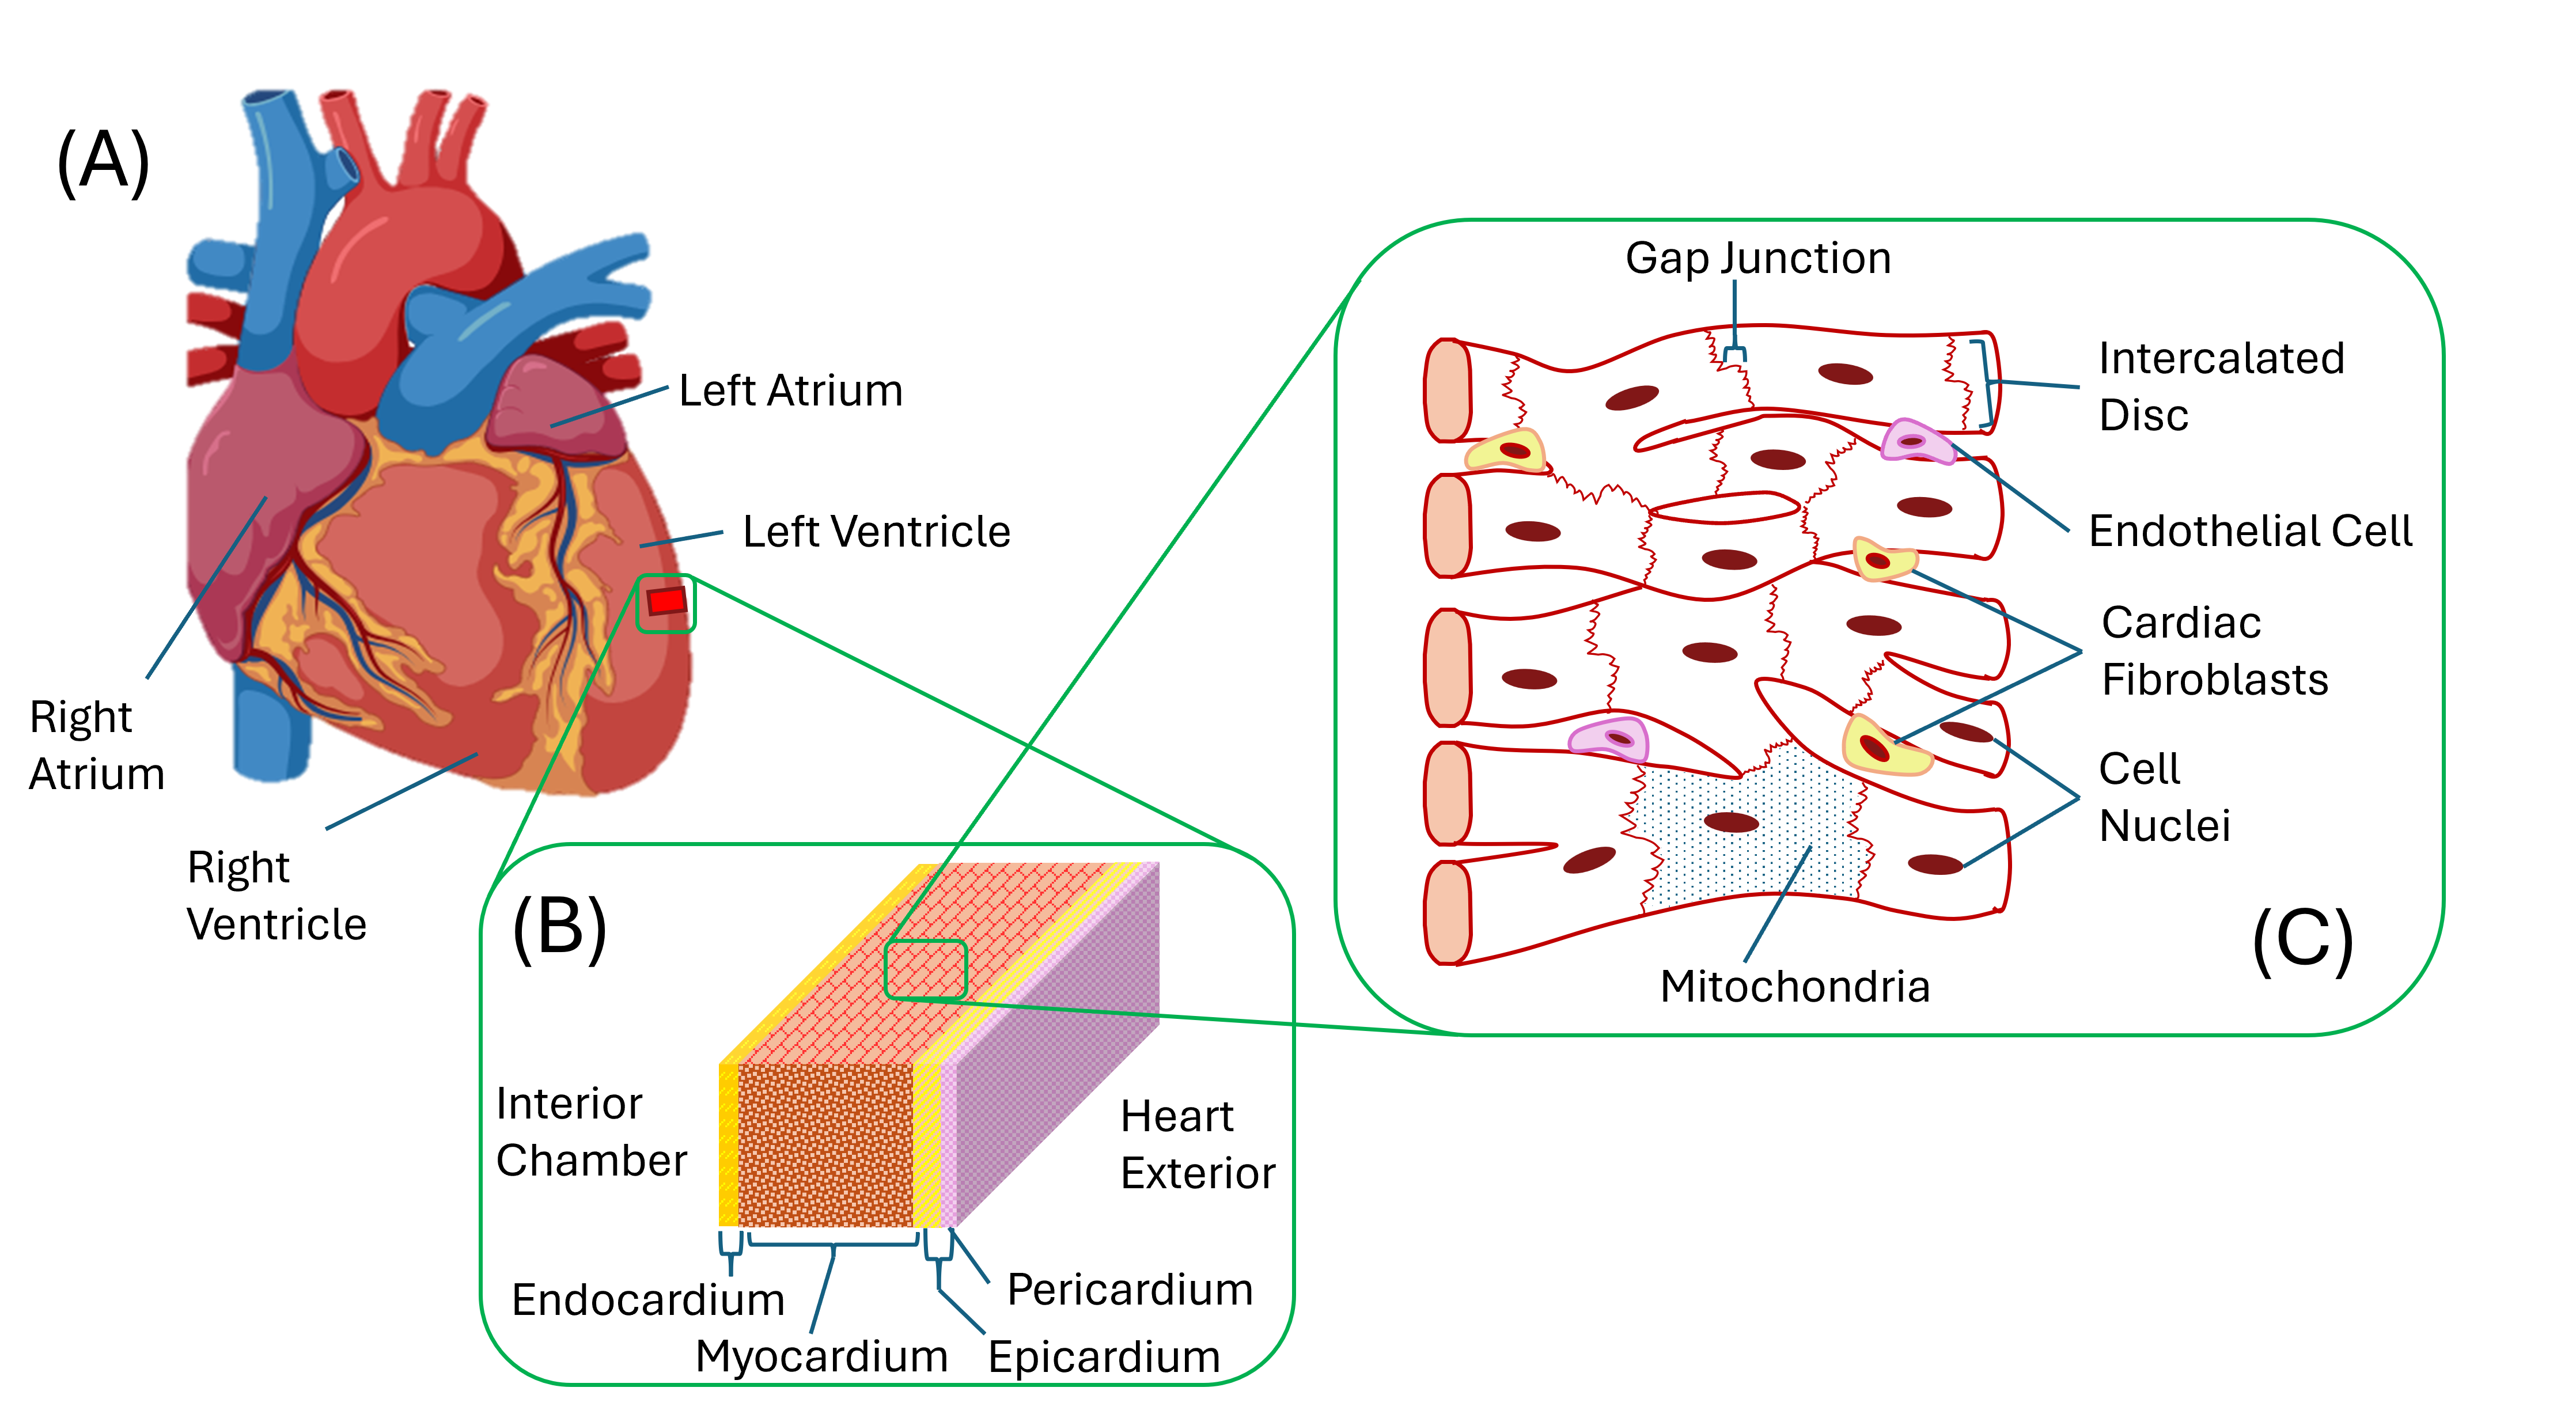
\includegraphics[width=0.85\linewidth]{Figures/Figure1.1.png}
    \caption{\textbf{Diagram of cardiac and cardiomyocyte structure and features}. Main figure details overall organ structure. Middle inset: structure of Left Ventricle (LV) wall in the organ, Left inset: structure of myocardium region in the LV wall. Created in  https://BioRender.com.}
    \label{fig:enter-label}
\end{figure}

Some of the key features that distinguish CMs from all other cell and muscle types in the body include: high concentrations of mitochondria (5,000-8,000 per cell), striated and branching cell shapes, connection to other CMs via intercalated discs and gap junctions []. These features, in combination with the use of ion channels and protein pumps in the cardiomyocyte membrane, enable cardiac tissue to maintain the high metabolic activity required for high speed, synchronized contraction without fatiguing \cite{woodcock_cardiomyocytes_2005}. 



\subsection{Cardiac Electrophysiology}
To perform this rhythmic contraction and relaxation of CMs in the heart, a sequence of electrical signals is transmitted to and throughout the organ via a network of nerve cells \cite{saltzman_biomedical_2015}. A diagram showing the path, key structures, and pattern of electrical depolarization across the heart to form the heart beat is shown in Figure \ref{fig:HeartElec}:

\begin{figure}[H]
    \centering
    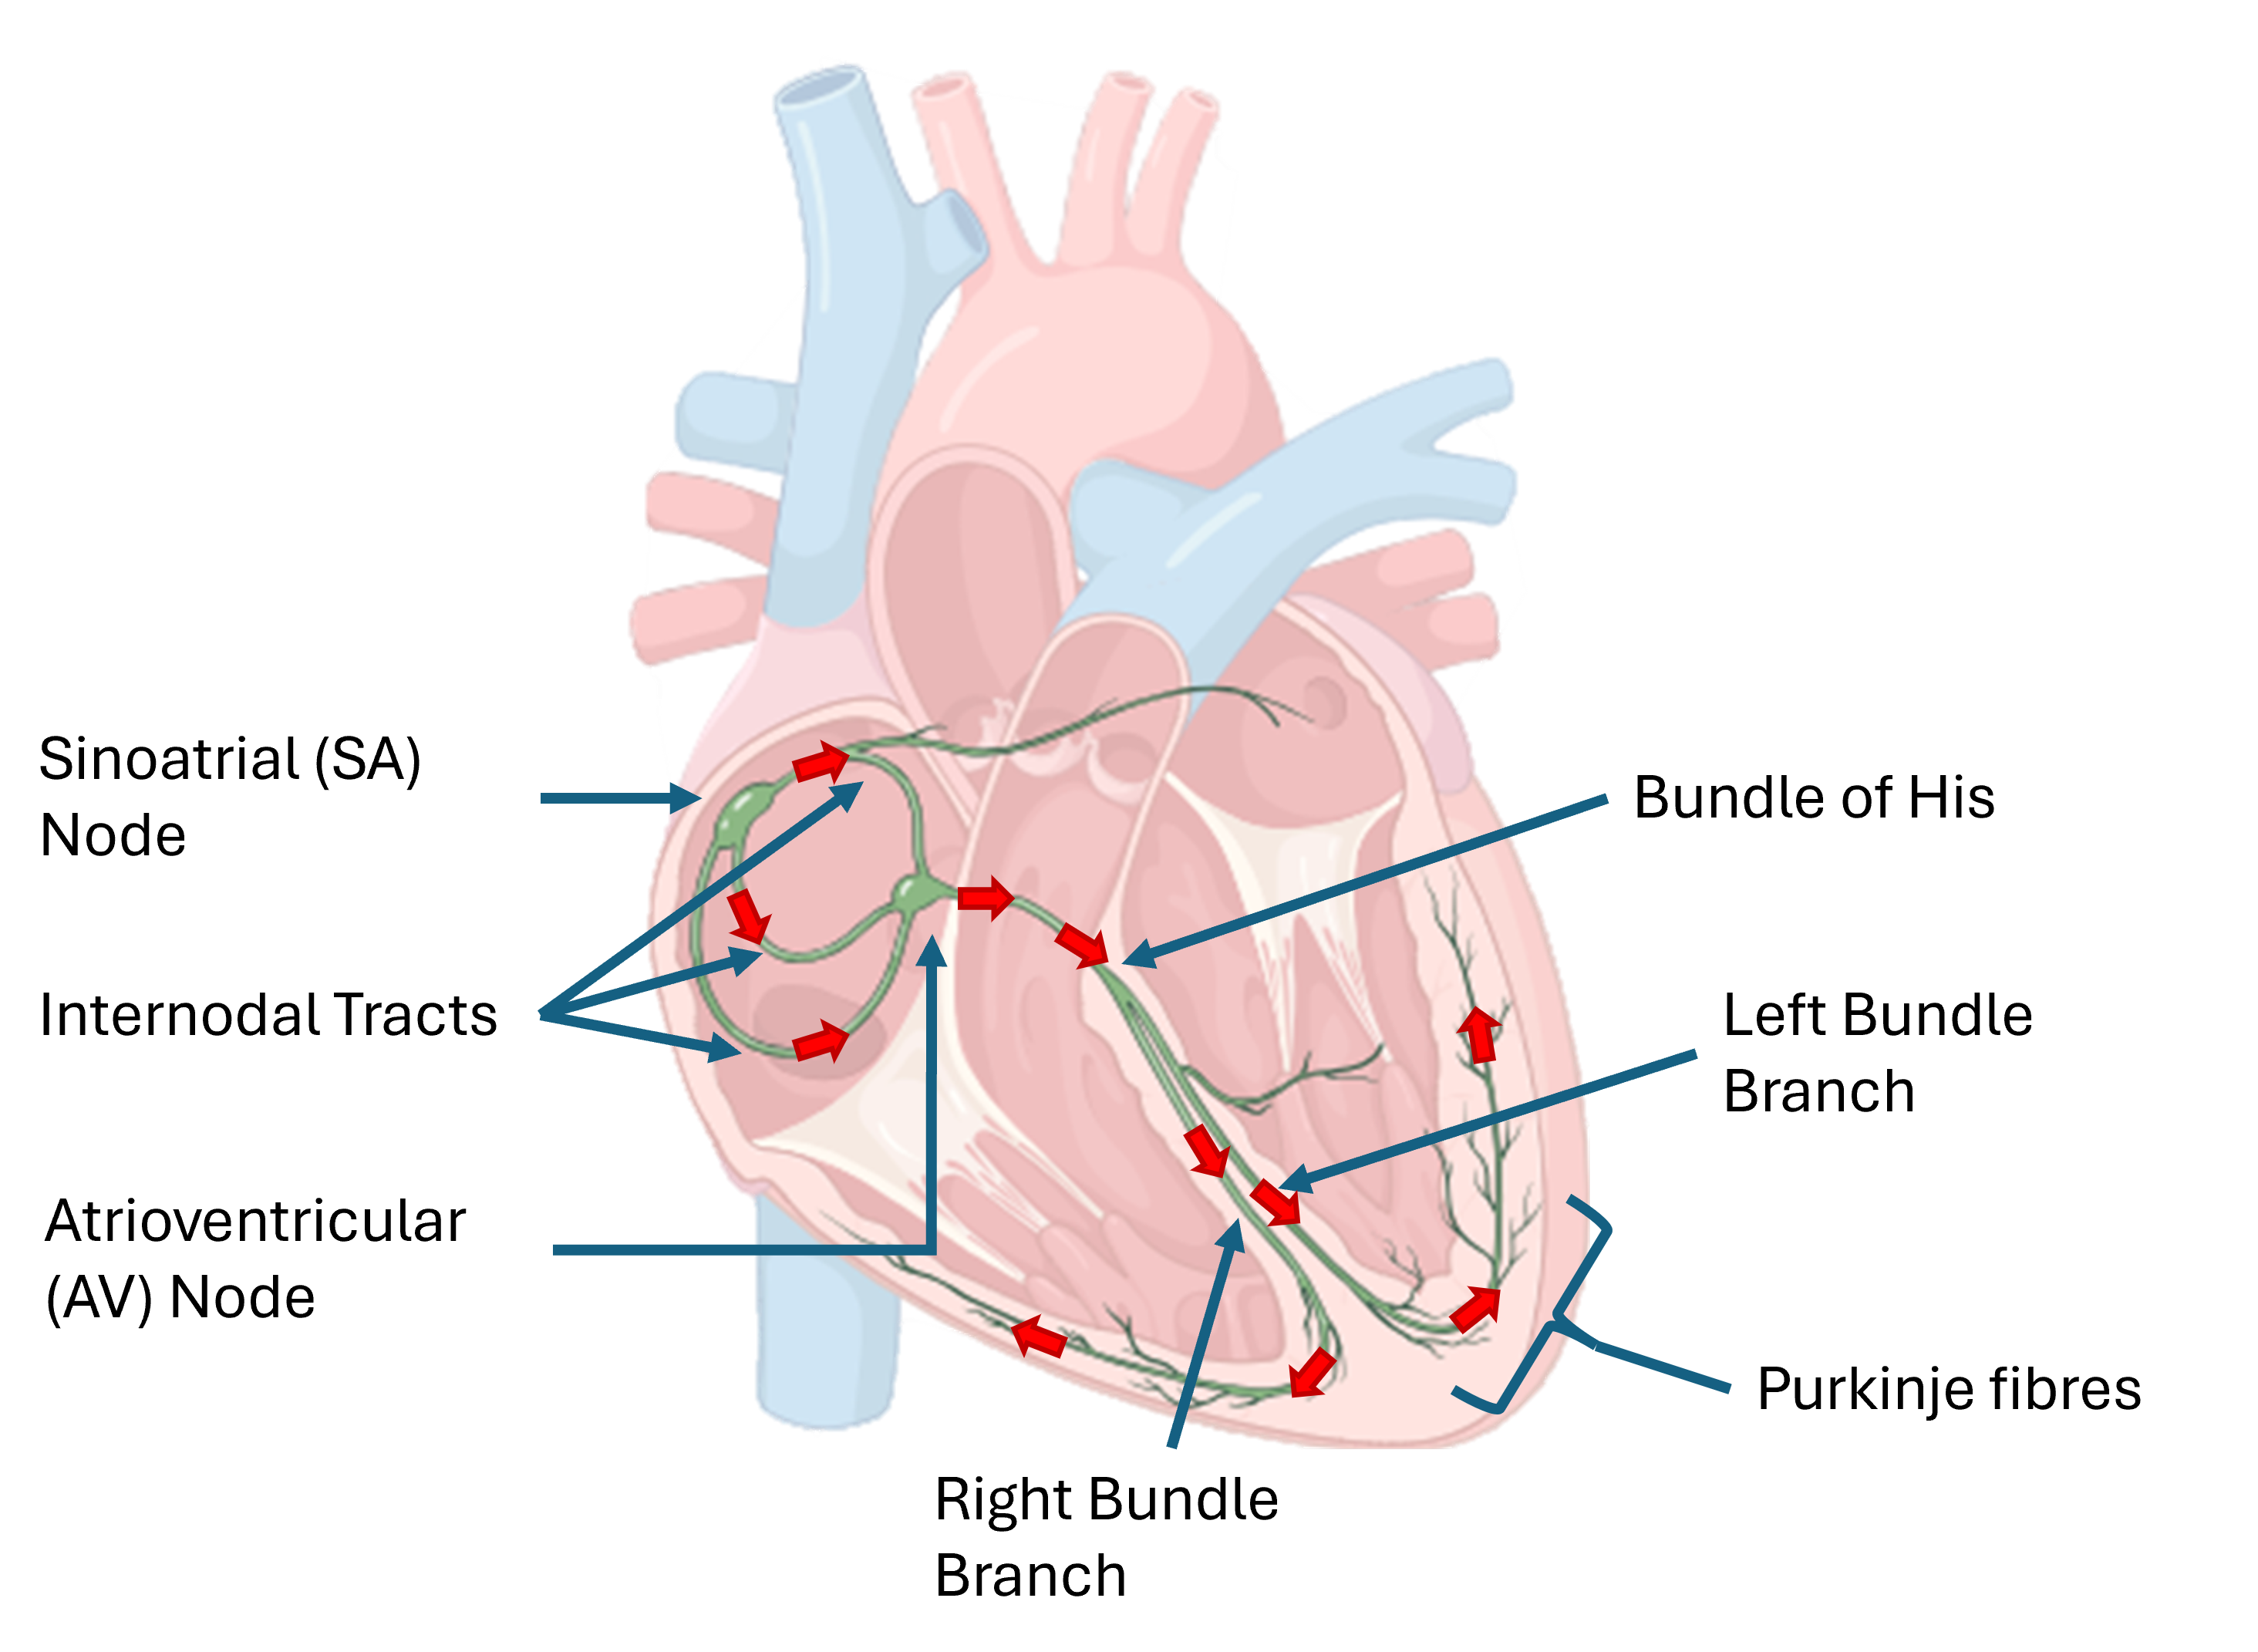
\includegraphics[width=0.85\linewidth]{Figures/Figure1.2.png}
    \caption{\textbf{Diagram of the heart and key structures for cardiac electrical activity.} Red arrows indicate direction of depolarization from SA Node to Perkinje Fibre network throughout the heart. Created in  https://BioRender.com. }
    \label{fig:HeartElec}
\end{figure}

Initiating signals generated by the sympathetic and parasympathetic nervous system is introduced to the organ at the Sinoatrial (SA) Node located in the right atrium chamber of the heart. The cells of the SA Node rhythmically depolarize in response to these signals originating from the brain[]. The depolarizing sequences then traverse the tissue of the right atrium via a series of internodal tracts to the Atrioventricular (AV) Node and the Bundle of His located near the centre of the heart. At the Bundle of His, depolarization progresses on to the upper corners of the ventricles closest to the bundle before then traversing down bundle branches and across the rest of the ventricular myocardium. The wave of depolarization across the myocardium concludes at the Perkinje fibre network at the end of the branch network \cite{saltzman_biomedical_2015}. All remaining cardiac tissue has depolarized by this point, which is followed immediately by repolarization of the myocardium in preparation for the next wave of depolarization \cite{saltzman_biomedical_2015}.

\subsection{Myocardial Infarction Alterations}

The need for rapid and perpetual repolarizing of cells in the myocardium requires massive investment of the CM metabolic activity and time. The consequence of devoting so much cell function to this feature is the cessation of other cellular activities commonly seen in eukaryotic cells. This includes the ability for these cells to replicate and repopulate by means of mitosis, which is possible to some extent in most other tissues in the human body. Skeletal muscles, red blood cells, and neurons are also incapable of replication, but all have alternative means of replacing lost or damaged cells such as the use of myosatellite cells in skeletal muscles, neuroplasticity in neurons, and red blood cell formation in bone marrow \cite{paxton_leeds_2003}. No such alternative exists for terminally differentiated CMs after the population of differentiable stem cells is depleted in early stages of human development \cite{uygur_mechanisms_2016}. 

 The process of tissue remodelling in the heart tissue is the result of myocardial infarctions (MIs). A MI is instigated in by a loss of blood flow to a region of the heart due, in most cases, to obstructions in the coronary vessels delivering oxygenated and nutrient rich blood to the myocardium. With no means of replacing or repairing lost or damaged tissue, the immune system of the body defaults instead to a process of cardiac remodelling to prevent the heart from bursting through the damaged region at the heart continues to pump blood \cite{huethorst_development_2022}.  Once the remodelling is complete, three unique regions in the cellular matrix of the heart muscle emerge \cite{huethorst_development_2022}. These regions, and features unique to each, are shown in Figure \ref{fig:postMI}. 

\begin{figure}[H]
    \centering
    \includegraphics[width=0.85\linewidth]{Figures/Figure1.3.png}
    \caption{\textbf{Diagram of heart tissue regions post-MI.} Close up inset legend: (A) MI heart healthy zone, (B) MI heart border zone, (C) MI heart scar zone. Created in  https://BioRender.com.}
    \label{fig:postMI}
\end{figure}

In the post-MI heart, healthy zones (Figure 1.3, Inset (A)) are the remaining regions of cardiac tissue that remain active and operation post-MI with the ability to contact and propagate electrical activity as normal. Conversely, Scar Zones (Figure 1.3, Inset (C)) are those regions of tissue where the CMs have died, being replaced with fibrotic scar tissue. This scar tissue has no ability to contract or propagate electrical activity. In between these two regions is the Border Zone (Figure 1.3, Inset (B)) which are regions that possess a mixture of active and deceased cells in varying ratios which still has limited, sporadic ability to contact and propagate electrical signals \cite{huethorst_development_2022}.

With their high metabolic demands, CMs undergo uncontrolled cell death, necrosis, quickly after being cut from their continuous supply of oxygen and nutrients \cite{huethorst_development_2022}. With each cardiomyocyte lost, the collective strength of the cardiac tissue degrades and the electrical activity that perpetuates rhythmic heart beating is interrupted as the dead cellular tissue is no longer able to perpetuate the waves of electrical depolarization to adjacent cells awaiting the signal to propagate the heart’s pumping activity. Should a sufficiently high number of CMs undergo necrosis, the ejection fraction of the heart will reduce to less than 40\% of the total blood in the heart, leading to heart failure. This failure is fatal without immediate medical treatment to restore or substitute cardiac activity and resume the flow of nutrient rich blood through the body \cite{golla_heart_2025}. 

The emergence of scar and border zones in the myocardium can also gradually introduce disturbances in heart rhythm, known as arrhythmias, that can increase in severity over time. The increase in severity stems from the scar region gradually stiffening over time, restraining movement of surrounding healthy tissue. The unregulated proliferation of nerve cells in border zones also gradually introduces disturbances in heart rhythms, leading to irregular patterns of depolarization to the surrounding healthy tissue that contribute to arrhythmia formation \cite{amoni_heterogeneity_2023, huethorst_development_2022}. Severe arrhythmias can eventually result in cardiac arrest should the irregular beat becomes too unstable and thus inefficient to pump sufficient blood throughout the body. This condition is highly lethal if not immediately treated and remains one of the leading causes of death for those living with hearts altered by MIs \cite{golla_heart_2025}.  




\section{Light Sheet Fluorescence Microscopy}
% REFERCES GIARDINI, OLIANTI THESES, mesoSPIM Paper

\subsection{Conceptual Premise}
To examine three dimensional structural changes in infracted hearts compared to healthy hearts, the imaging technique utilized must be capable of recording images of large volumes of tissue in reasonable amounts of time and with high, consistent spatial resolution. This leads to the selection Light Sheet Fluorescence Microscopy (LSFM) as the optical imaging technique of choice for this application.  

The main principle behind LSFM is the idea of using perpendicular pathways in excitation and detection to permit the simultaneous illumination and observation of a narrow plane of space across the system’s field of view \cite{voigt_mesospim_2019}. The excitation path consists of a Gaussian beam that uses galvanometer mirrors to shift the beam laterally to form the light sheet of the system. The basic setup of this method and a detailed look of the Gaussian beam and associated dimensions are shown in Figure 1.4.

\begin{figure}[H]
    \centering
    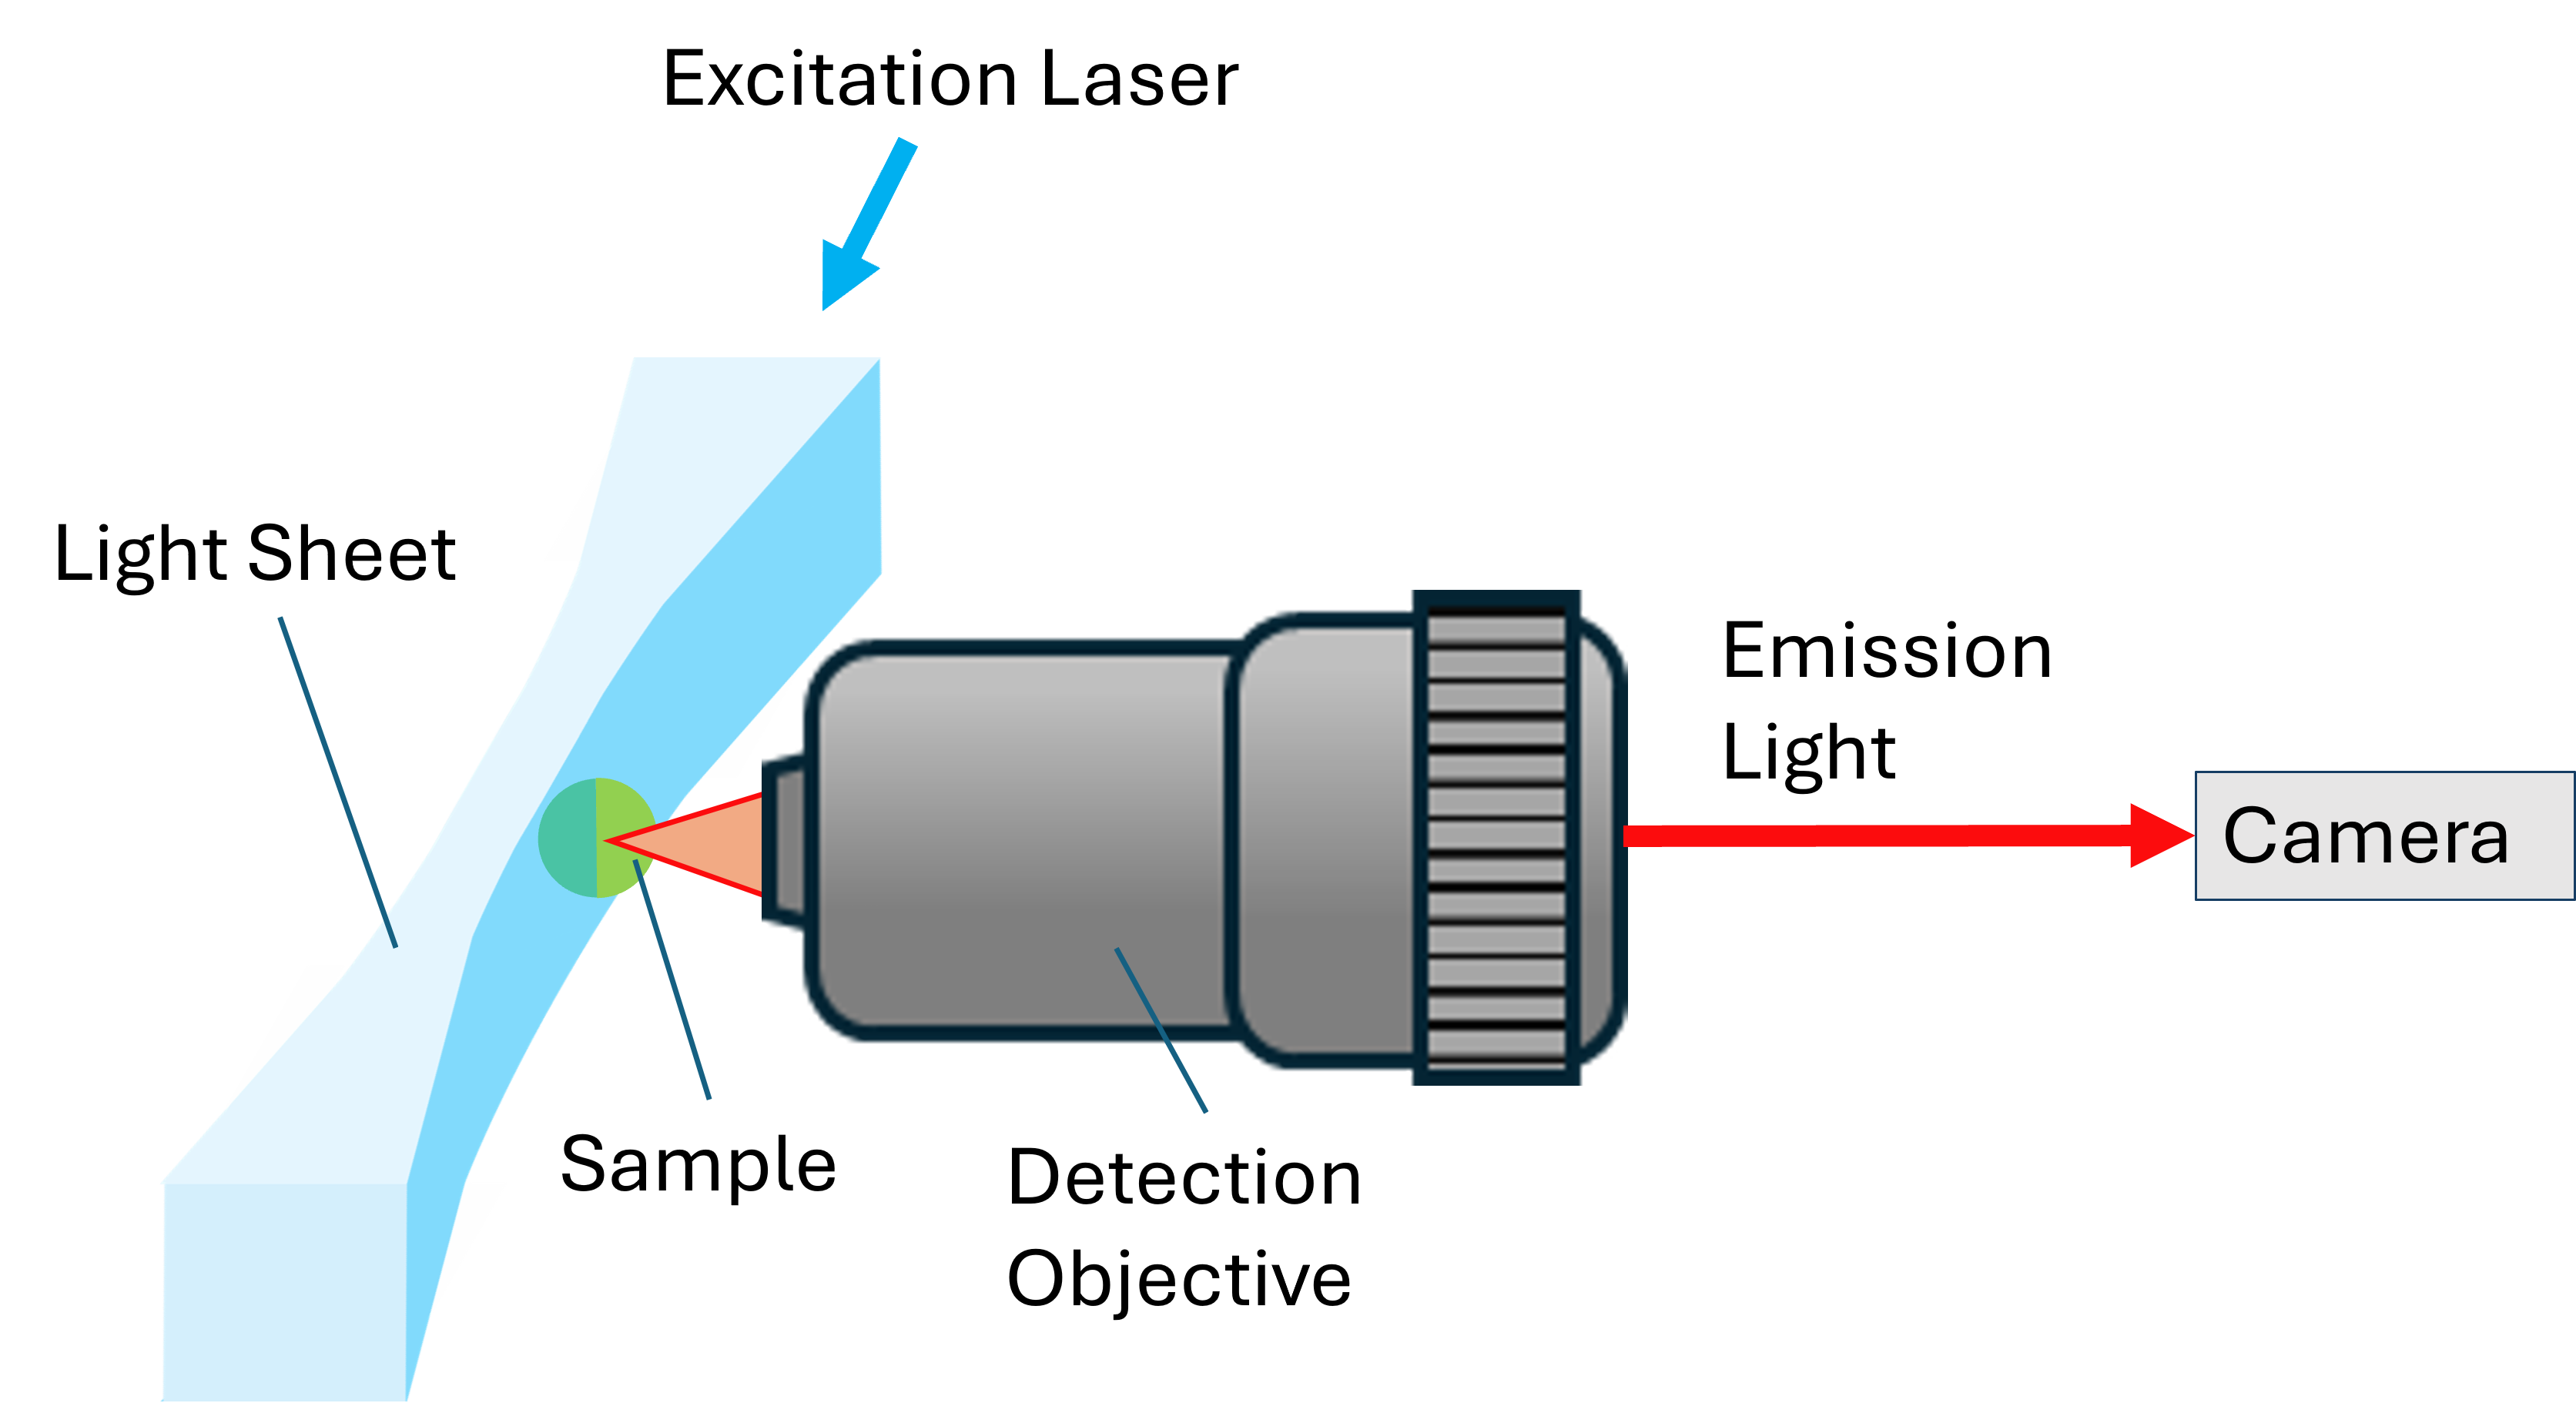
\includegraphics[width=0.75\linewidth]{Figures/Figure1.4.png}
    \caption{\textbf{Optical Diagram and Associated Components of Light Sheet Fluorescence Microscopy (LSFM).}}
    \label{fig:enter-label}
\end{figure}

When fluorescently stained samples traverse the plane of the light sheet, that plane of tissue will be illuminated and can be viewed by the scientific camera with high contrast, while the remainder of the sample remains unilluminated and not visible. The sample can then be shifted through the light sheet with the camera capturing images of each plane of the sample, recording the entire volume into a single image stack for use in analysis.

In theory, this microscopy concept can generate multiple thin slices images of a sample with high resolution and optical sectioning. LSFM is also capable of recording this data in relatively short periods of time as the separation of the excitation and emission pathways allows signal across the entire FOV to be recorded simultaneously rather than in sections \cite{poola_light_2019}. These image collections can then be recombined digitally to obtain a full three-dimensional image of the sample recorded. The ability to image across the volume without the need for excision or slicing has the added benefit of preserving any structural features that would otherwise be lost in the process of sectioning the tissue to conform to more standardized methods of microscopy.

An additional benefit to this microscopy method is the reduction of photobleaching and phototoxicity that can occur in tissue samples due to overexposure to high powered sources of illumination. By expanding the illumination from a singular point to across an entire plane of the imaging, the intensity of the emitted light is diluted, allowing for longer imaging sessions to occur more frequently with reduced risk of damage to the tissue or loss of fluorescence after repeated. excitation.

\subsection{Axially Scanned Light Sheet}
The use of a light sheet to illuminate a thin plane across the field of view can also have the added benefit of being capable of generating homogenous resolution images across large fields of view. This can be achieved through the technique called Axial Scanning Light-sheet Microscopy (ASLM). This technique takes advantage of the unique characteristics of the Gaussian Beam, which is detailed in Figure \ref{gb}.

\begin{figure}[H]
    \centering
    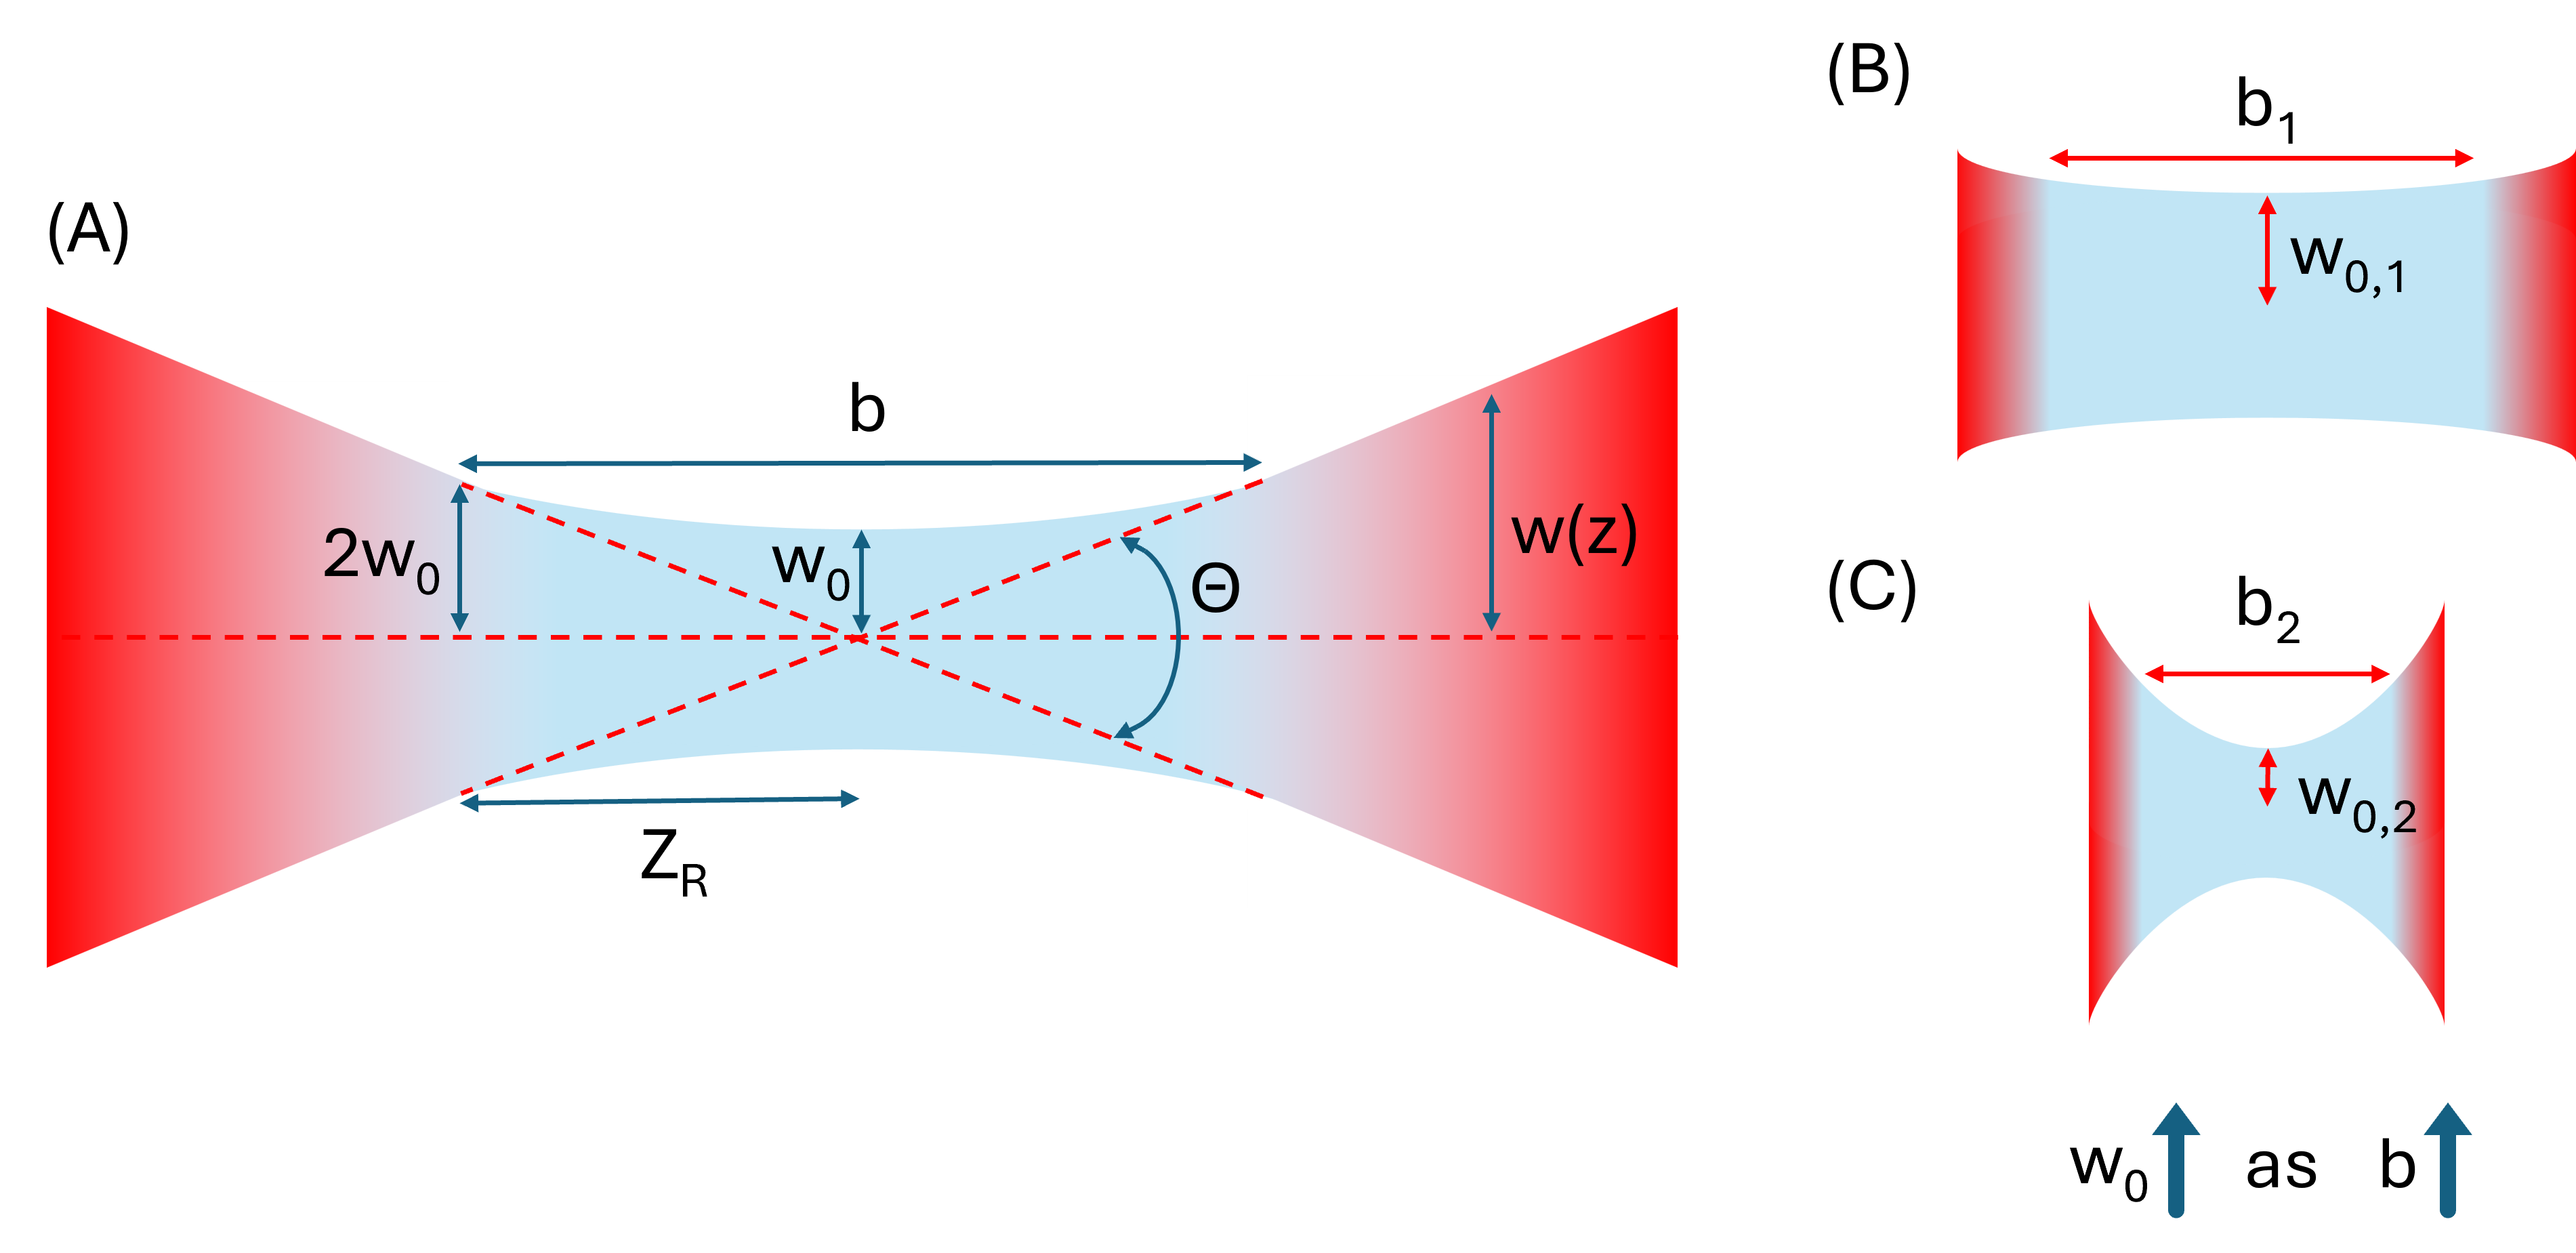
\includegraphics[width=0.85\linewidth]{Figures/GaussianProfileDiagram.png}
    \caption{\textbf{LSFM Gaussian Beam Profile.} Legend: \(w_0\)= Beam Waist, \(Z_R\) = Rayleigh Length, b = Depth of Focus, w(z)= Gaussian Beam Width, \(\theta \) = Total Angular Spread. Beam region within depth of focus range highlighted in cyan. Insets (B),(C) showcase relation between $w_0$ and b.\cite{paschotta_gaussian_2005}}
    \label{fig:gb}\
\end{figure}

The thickness of the Gaussian beam follows a well established characterization formula: 

\begin{equation}
w(z) = w_0 \sqrt((1+(\frac{z}{z_R})^2)
\end{equation}
\medskip

The minimum thickness of the Gaussian beam is located at the beam waist ($w_0$) and its relation to the light wavelength and the Numerical Aperture (NA) of the Excitation pathway is given by:

\begin{equation}
w_0 = \frac{\lambda}{NA*\pi}
\end{equation}
\medskip

Similarly, the Depth of Focus (b) spans across the beam and defines the region where the the bean thickness (w(z)) is similar enough in value to the beam waist to be considered consistently concentrated for use in acquiring homogenously resolved images \cite{paschotta_gaussian_2005}. The depth of focus relation to the beam waist is given by:

\begin{equation}
b = \frac{2\pi w_0^2}{\lambda}
\end{equation}
\medskip

Due to these interconnected relations between the NA, depth of focus, and beam waist, it is possible to expand or reduce the dimensions of the beam by adjusting the NA of the excitation pathway. As shown in insets (B,C) of \ref{gb}: decreasing the NA of the system, the depth of focus will increase but at the cost of increasing the beam waist, lowering the resolution the beam can resolve the process. Conversely: by increasing the NA, the beam waist can be reduced to record at higher resolutions but at the cost of shortening the depths of focus. While the LSFM system will be able to record at higher resolution with a high excitation NA, it will only be able to do so in the central region of the camera FOV as the depth of focus will no longer span the length of the FOV. This leaves the left and right sides of frames recorded at a low resolution compared to the middle. ASLM resolves this issue to generate homogenously resolved images by utilizing tuneable lenses and camera rolling shutters as diagrammed in Figure \ref{aslm}. 

\begin{figure}[H]
    \centering
    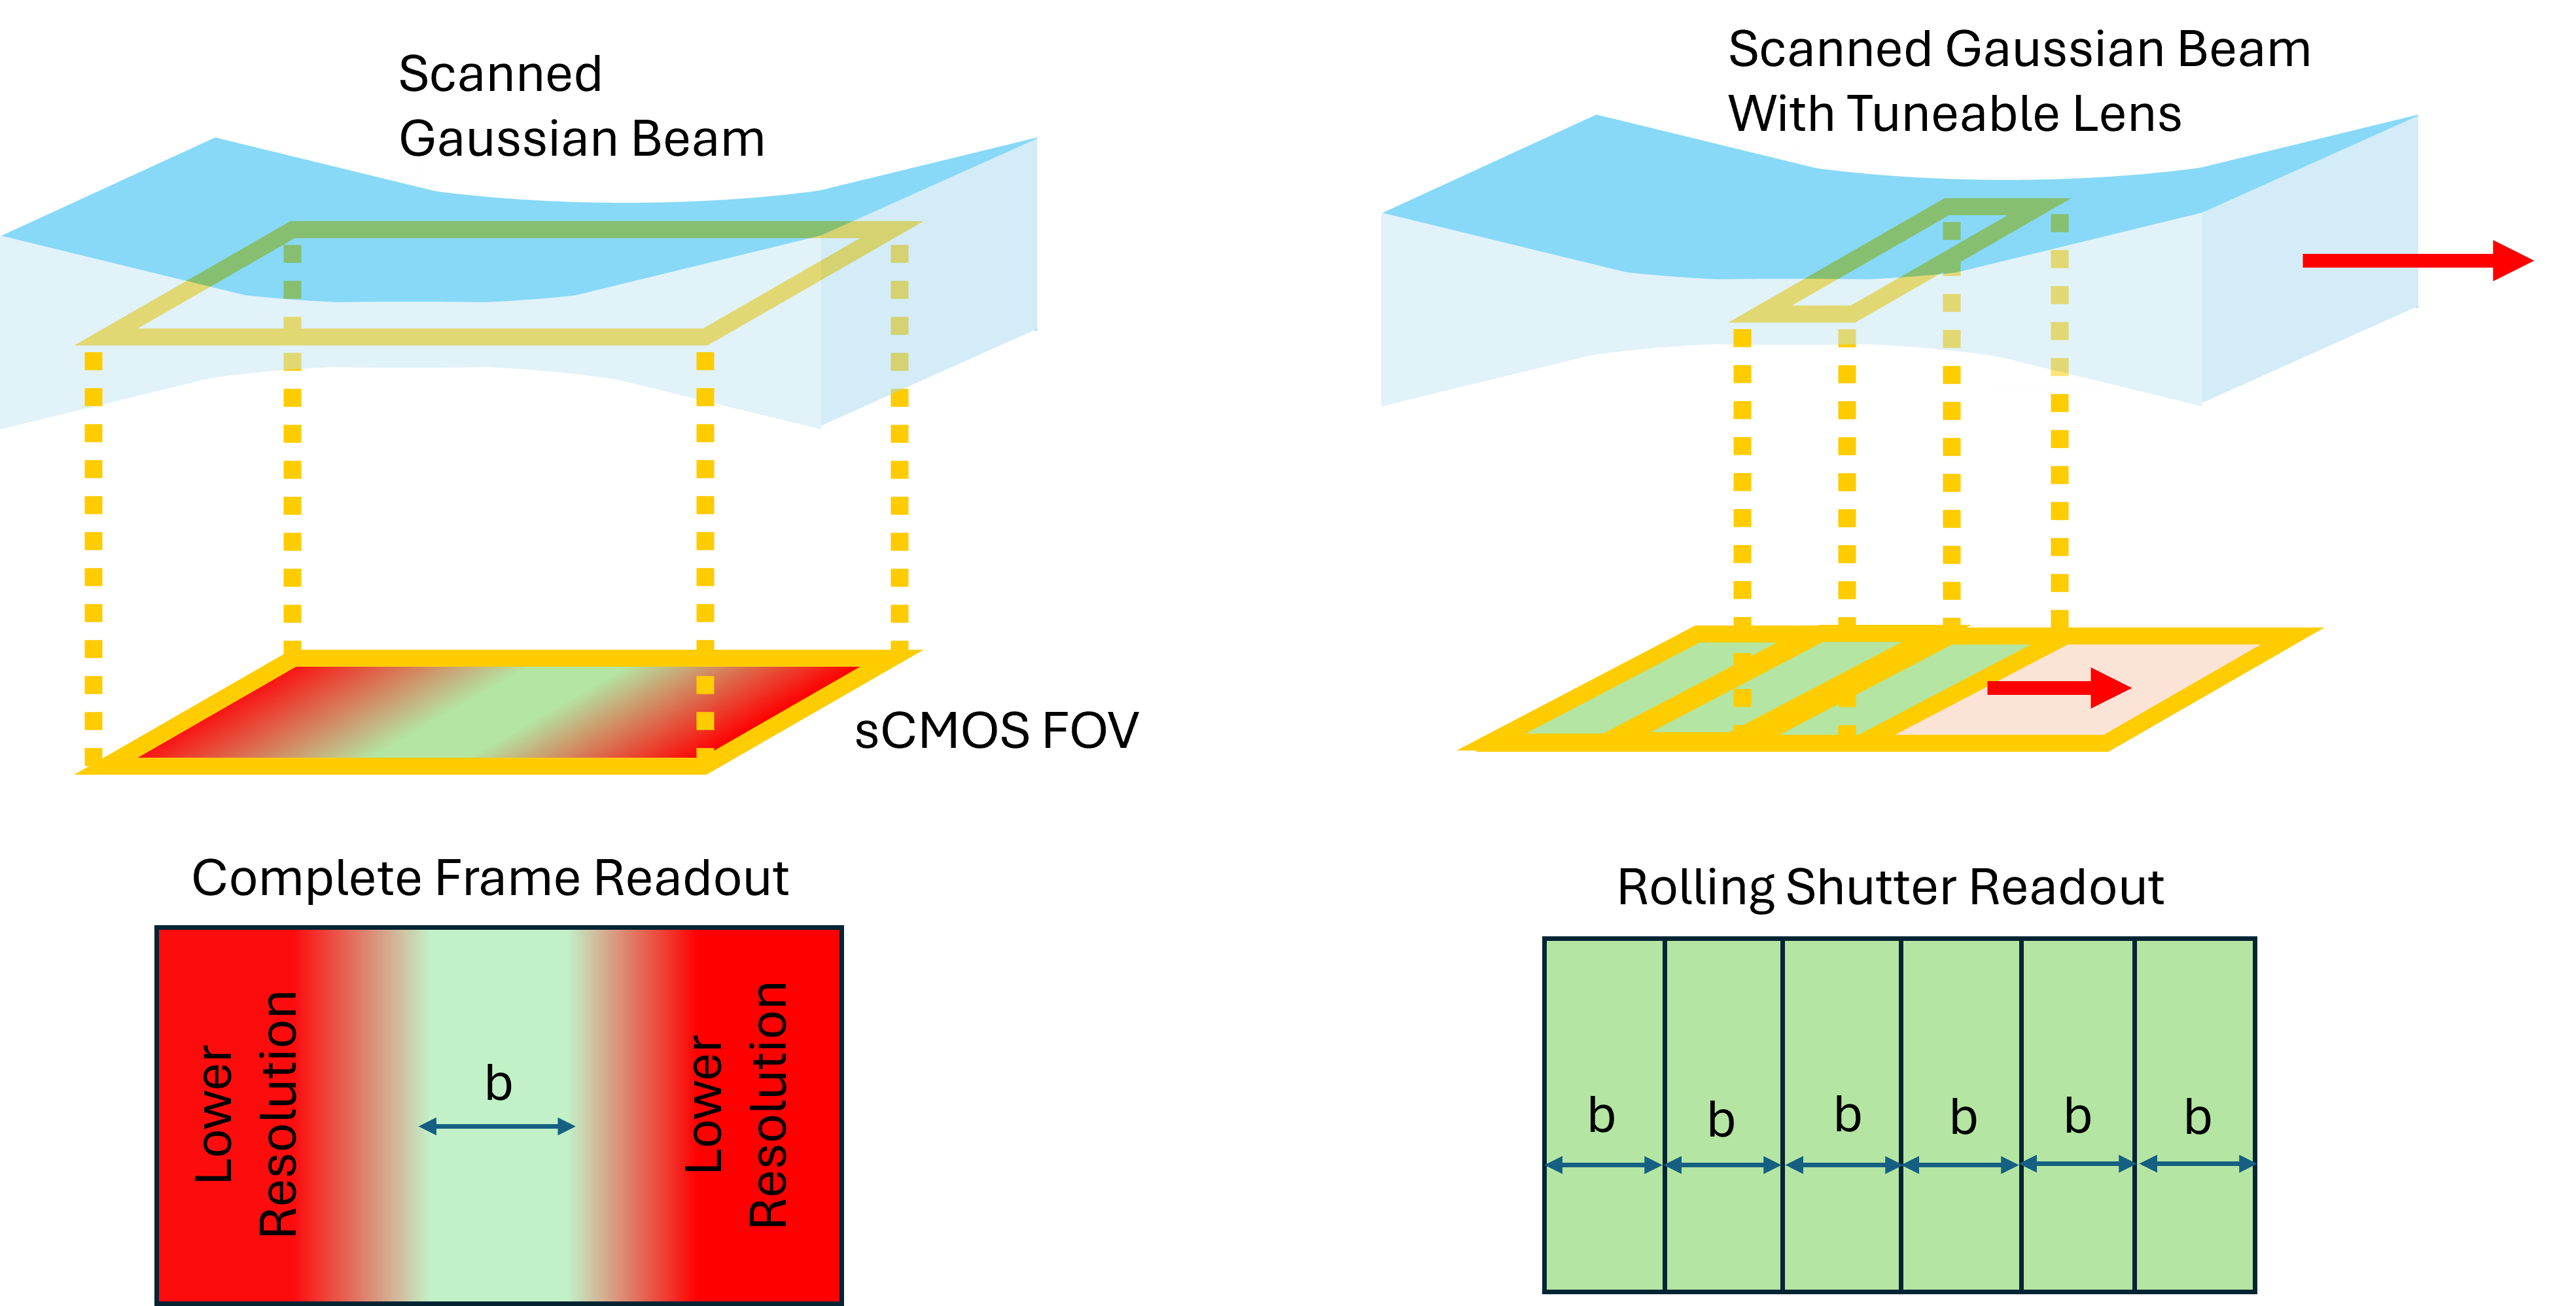
\includegraphics[width=0.85\linewidth]{Figures/ASLMDiagram.png}
    \caption{\textbf{Diagram of ASLM Imaging Technique.} Comparison of Traditional (left) and Axial Scanned (right) Light Sheet Image Acquisition. Region of Light Sheet Within Depth of Focus (b) Labelled, Shown In Green}
    \label{fig:aslm}\
\end{figure}

By synchronizing the camera rolling shutter to the shifting of the beam waist across the frame, the scientific camera will record the narrow spans of pixels in the frame where the beam waist is located as it shifts locations \cite{voigt_mesospim_2019}. The camera will then digitally combine all of these narrow spans together into a complete frame covering the entire FOV, forming an image in which the beam waist is present across the entire image and therefore is homogeneously resolved. 

\subsection{Practical Limitations}

Light Sheet Microscopy techniques, of both traditional and axial scanned variations, have two obvious limitation which impairs the usability of this method for volumetric imaging of tissue samples: 

\begin{enumerate}
    \item Vast majority of LSFM systems in use today are incapable of accommodating thicker, non sectioned samples \cite{poola_light_2019}.
    \item Tissues found in biology are insufficiently transparent to allow optical sectioning to occur \cite{olianti_optical_2021}.
\end{enumerate}

\subsubsection{Tissue Volume in LSFM Systems}
Most LSFM systems developed and made commercially available are unable to accommodate larger volume samples that are not physically sectioned into micron thick slices. This is due to the complicated hardware and optical pathways surrounding the sample making manipulation of samples across light sheets for distances greater a few millimetres extremely difficult \cite{krzic_multiview_2012, poola_light_2019, gualda_openspinmicroscopy_2013}. To compound the problem, due to the relation between the Gaussian beam waist and the depth of focus, to obtain the highest resolutions possible, the usable region of the light sheet will be incredibly narrow even with the application of ASLM into the system. This will result in the need for image tiles numbering in the hundreds of tiles to cover samples with large surface areas, making complete reconstruction of tissue volumes extremely time consuming and computer process intensive to complete \cite{poola_light_2019}.

\subsubsection{Tissue Transparency in LSFM Systems}
 The second issue encountered when attempting to image mesoscale samples comes from the opacity of the tissues themselves. Even if the Gaussian beam is sufficiently powerful for the light sheet to successfully penetrate across the tissue, any fluorescent emission created as a result will not be intense enough to exit back out of the tissue towards the detection objective and camera. There is also the possibility for such high power light to cause damage to the tissue and quench the fluorescence of dyes in the sample, rendering the tissue incapable of producing images of any degree of quality regardless of the tissue's opacity.

This opacity stems from the refractive index (RI) mismatch between the various biomolecules inside the tissue (lipids, proteins, blood, water, et cetera) and the surrounding external environment (atmospheric air) \cite{paysan_art_2023}. This optical metric quantifies the reduction in speed experienced by incident light when propagated through a given medium. Sudden changes in RI that can occur as light travels across two mediums can severely hinder the propagation of light, leading to an increase in light scattering and in turn increase the opacity of the medium the light enters.

The sudden and drastic change in RI between air (RI $\approx$ 1.0) and cardiac tissue ( RI $\approx$ 1.382) will scatter the light upon contact to the tissue surface, preventing the Gaussian beam from forming the desired beam waist. Traditionally, in biological histology, the solution to this issue would be to physically slice samples into extremely thin slices, defeating the purpose of using the LSFM technique for volumetric imaging. To solve this issue without sectioning the tissue, several LSFM systems have implemented engineered excitation beams such as Bessel, airy, and lattice beams to reduce scattering and improve penetration into the tissue volume without light diffraction \cite{sapoznik_single-objective_2020, poola_light_2019}. This method of tissue clearing is the preferred methods to overcoming this obstacle with respect to large volume imaging as the use of engineered beams in LSFM requires mechanically complex and costly setups which limit the viability of wide scale use in research. As a result, instead of changing the beam utilized, the preferred method of choice to overcome this obstacle is to change the tissue itself via chemical treatments to increase the transparency of the tissue. This form of chemical treatment, known as tissue clearing, allows the Gaussian beam to traverse the sample with lower light scattering and absorption. 


\section{Tissue Clearing Protocols}
\subsection{Conceptual Premise}
Chemical treatment of biological tissues to render them translucent or even fully transparent has been a field of research explored by researchers for well over a century \cite{paysan_art_2023}. The technique of tissue clearing aims to homogenize the RI of tissues composed of heterogenously organized biomolecules. The biomolecules most influential to the RI mismatch of tissues to its ex situ environment include water (RI = 1.33), lipids ($RI \approx 1.44$), and proteins ($RI \approx 1.43$). To achieve closer (if not near perfect) RI homogeneity, clearing processes seek to remove, alter, and/or replace one or more of these biomolecules from the tissue without altering the existing internal structure. This will allow the remaining molecules of similar RI to be matched to the RI of the external environment via immersion into a solution with an equal RI value \cite{paysan_art_2023, tainaka_chemical_2018}. Fully immersed, the entire sample volume will now be fully RI matched and can hereafter be imaged with LSFM, taking advantage of the techniques optical sectioning with no further hindrance. An example of how effective tissue clearing can be in rendering tissues optically transparent, a before and after comparison photo showcasing a tissue before clearing, after clearing, and after immersion in RI matched solution is shown in the following Figure:

\begin{figure}[H]
    \centering
    \includegraphics[width=0.85\linewidth]{Figures/Figure1.7.png}
    \caption{\textbf{Tissue Transparency Before and After Tissue Clearing.} 400 micron thick Leporine tissue slice before clearing (A), after clearing (B), and after RI matched solution immersion (C). Sample processed using CLARITY method of tissue clearing (see section 3.2 of this chapter).}
    \label{fig:enter-label}\
\end{figure}

\subsection{Methodology Variations}


Three categories of clearing methodologies have emerged which utilize unique chemical processes to achieve RI matching of tissue to their \textit{ex vivo} environment. Each of these categories (dehydrating, hyper-hydrating, and hydrogel-hybridizing) have unique advantages and disadvantages to each in addition to containing a wide variety of sub-categories and variations that fall under the umbrella of each category \cite{paysan_art_2023}. This wide range of clearing options is also perpetually expanding in size as new methods and variants are published in this field on a regular basis. 

\subsubsection{\textit{Dehydration Methods}}
Dehydration methods of tissue clearing utilizes alcohol solution immersion to dehydrate the tissue, raising the RI as water is expelled along with dissolved lipids \cite{paysan_art_2023}. Samples thereafter are immersed in an organic solvent with an RI matching that of proteins in the tissue. This solvent removes any remaining lipids as it intercalates with the cellular structures inside the tissue. With the solvent now replacing the water and lipids in the tissue structure, the RI has been homogenized to the solvent and rendered transparent. 

While simplistic and fast to perform to completion, the dehydration method causes considerable alteration to tissue structure \textit{ex vivo} \cite{olianti_optical_2021}. This makes analysis of the cleared tissue structure unviable for biological analysis as the structure should be preserved as close as possible to \textit{in vivo} conditions. Doing so will allow for the most accurate insight into the biological activity of interest to be obtained.

\subsubsection{\textit{Hyper-hydrating Methods}}
Methods of the hyper-hydrating (or hydrophilic in some publications) variety utilize non-hydrophobic detergent solutions to extract lipids from the sample. This occurs as a result of an osmotic gradient that forms inside the tissue cellular structures, allowing water to penetrate into regions of the cells it would not normally be able to reach \cite{paysan_art_2023}. As lipids gradually diffuse out of the tissue, the structure remains mostly intact (depending on the detergents used) and expands in volume with the retention of additional water. This expansion is mitigated once the sample is removed from the detergent and placed in a RI matching solution (RIMS), expelling the water, being replaced with the intercalating solution that homogenizes the remaining tissue to its RI.

Hyper-hydrating methods of clearing can vary wildly in quality and in their ability to preserve tissue structure. Numerous combinations of detergents, alcohols, and solvents have been tested with certain combinations performing well with certain tissue types and poorly in others \cite{paysan_art_2023, olianti_optical_2021, susaki_whole-brain_2014}. Careful consideration is therefore required in selecting a specific method in this category, with through testing performed beforehand to confirm the viability of a method for use in clearing a specific tissue type with minimal alteration to in situ structure. 

\paragraph{CUBIC: Cleared Unobstructed Body Imaging Cocktails}
Of the hyper-hydrating methods of tissue clearing, the CUBIC family of clearing protocols provide some of the best clearing results among hyper-hydrating methods with minimal alteration to tissue structure after completion of the process \cite{susaki_whole-brain_2014, tainaka_chemical_2018}. Several variations of of the CUBIC protocol have been developed and made commercially available since the initial publication in 2014 by the CUBIC Stars team at the University of Tokyo. These cocktail varieties allow the protocol to be used with a variety or combination of tissue types up to and including entire animal bodies \cite{noauthor_cubic_nodate}. The CUBIC second generation variant, CUBIC-L/RA, is one such protocol that has been shown in previous publications by the developers and independent researchers to have the best capability among the CUBIC family of chemical cocktails to clear cardiomyocyte samples with minimal structural change and preservation of dye fluorescence after immersion in RIMS \cite{tainaka_chemical_2018}. As such, this makes CUBIC-L/RA the most optimal choices on the market today for cardiomyocyte clearing by hyper-hydrating means. 

\subsubsection{\textit{Hydrogel-Hybridizing Methods}}
Developments in past decade has led to the rise in the use and efficiency of methods which remove entire categories of molecules from tissue samples. In their place, these methods create hydrogel matrices that maintain the structure of the sample without the RI mismatch of the original molecules \cite{paysan_art_2023}. This is achieved by exposing tissue samples to monomers and a fixative chemical which induces a polymerized hydrogel mesh to be formed across the tissue volume. The matrix serves a scaffold holding proteins and other molecules of interest in position while allowing unwanted molecules causing RI mismatch, such as lipids, to be removed from the tissue using highly concentrated detergent solutions. Immersion in RIMS will complete the clearing process with the hydrogel-hybridized tissue quickly homogenizing to the solution. Hydrogel-Hybridized methods are capable of rendering tissue transparent to the point of becoming invisible to the human eye when immersed in RIMS. As such, techniques based in this method are well regarded in the research field as producing the highest quality tissue clearing achievable today. 

One major issue present in many hydrogel-hybridizing methods is that they tend to decrease the structural stability of the tissue as the hydrogel matrix which preserves the tissue structure is itself highly gelatinous. Cleared samples can be damaged easily when handling of the sample. As the sample acquires a slippery, gelatinous condition after clearing, the additional fragility makes handling of these tissue extremely difficult and time consuming. Further complicating adoption of these methods for use in research is the fact that the processes of polymerizing the acrylamide polymer and removing lipids from the tissue can be very complex and time consuming to properly complete. Specialized equipment including (but not limited to) pressurized gas, vacuum chambers, fume hoods, and safety gear can be required to properly polymerize the monomer \cite{olianti_optical_2021}. Detergent clearing, while simpler to perform compared to polymerization, can require several weeks to months to complete depending on the tissue type and volume .

\paragraph{CLARITY: Clear Lipid-exchanged Acrylamide-hybridized Rigid Imaging Tissue Hydrogel}

The most prominent hydrogel-hybridizing methods of tissue clearing is the CLARITY method, which utilizes a combination of acrylamide and bis-acrylamide monomers to form the hydrogel mesh via polymerization in Nitrogen gas . The lipids of the sample can then be removed by immersion in a solution of Sodium Doedecyl-Sulfate (SDS) over the course of 4 to 6 months\cite{olianti_optical_2021}. The cleared tissue could then be RI matched using a proprietary RIMS solution designed specifically to match with the RI of CLARITY cleared samples.  While the process is extremely time consuming and complex to perform, previous results achieved using the method with cardiomyocyte samples still makes the CLARITY methods one of most effective clearing protocols for cardiac tissue clearing in use today \cite{paysan_art_2023,olianti_optical_2021}. 

\section{Chapter Summary}

This chapter has set out to present the primary aim of this project: the development and successful application of a novel tissue imaging pipeline for use in structural analysis of cardiac tissue samples for use in cardiovascular research. The unique features and characteristics of cardiac tissue have been detailed here, explaining the processes by which structural modification as a result of MIs occur and proceed to degrade cardiac function over time. The importance of better understanding how these alterations occurred in the 3D structure of the myocardium is made evident and the means by which this information can be acquired is detailed in sections 1.2-3. Light Sheet Fluorescence Microscopy, in combination with Tissue Clearing Techniques, provides a basis by which the 3D volumetric imaging of cardiac tissue samples can be accomplished. To do this, an appropriate LSFM system, which is capable of overcoming limitations previously described in most LSFM systems, must be selected, assembled, and optimized for use in this newly formed imaging pipeline. This is the focus of the next chapter, which will also detail the acquisition, processing, storage of data recorded from the microscope into the PC for use in subsequent image analysis. 


